\documentclass[12pt]{article}

\usepackage[
    a4paper, 
    margin=2.5cm]{geometry}
\usepackage[utf8]{inputenc}
\usepackage[slovene]{babel}
\usepackage[
    pdfusetitle, 
    hidelinks, 
    unicode]{hyperref}
\usepackage{microtype}
\emergencystretch=1em
\usepackage{enumitem}
\usepackage{graphicx}
\usepackage{listings}
\usepackage{xcolor}
\usepackage[font=small]{caption}
\usepackage{times}
\usepackage{tikz}
\usepackage{amsmath}
\usepackage{amsfonts}
\usepackage{datetime}
\usepackage{booktabs}
\usepackage{array}
\usepackage{fancyhdr}
\usepackage[style=ieee, maxbibnames=3, minbibnames=1,
    maxcitenames=1, mincitenames=1, sorting=nyt]{biblatex}
\addbibresource{viri.bib}

\urlstyle{rm}

\setlength{\parindent}{0em}
\setlength{\parskip}{1ex}

\setcounter{secnumdepth}{5}
\setcounter{tocdepth}{3}

\renewcommand{\thesection}{\arabic{section}}
\renewcommand{\thesubsection}{\thesection.\arabic{subsection}}
\renewcommand{\thesubsubsection}{\thesubsection.\arabic{subsubsection}}

\renewcommand{\labelnamepunct}{\addcomma\space}
\DeclareFieldFormat[article]{title}{#1}
\DeclareFieldFormat[online]{title}{\mkbibemph{#1}}

\DefineBibliographyStrings{slovene}{
  andothers = {et. al\adddot},
  urlseen = {dostopano:}
}

\newdateformat{MMYYYYdate}{\monthname[\THEMONTH] \THEYEAR}

% Listings styling
\definecolor{codegray}{rgb}{0.95,0.95,0.95}
\definecolor{codegreen}{rgb}{0.1,0.5,0.1}
\definecolor{codeblue}{rgb}{0.1,0.1,0.7}
\definecolor{codepurple}{rgb}{0.5,0.0,0.5}

\lstdefinestyle{jsstyle}{
  backgroundcolor=\color{codegray},
  commentstyle=\color{codegreen},
  keywordstyle=\color{codeblue},
  stringstyle=\color{codepurple},
  basicstyle=\ttfamily\footnotesize,
  breakatwhitespace=false,
  breaklines=true,
  captionpos=b,
  keepspaces=true,
  showspaces=false,
  showstringspaces=false,
  showtabs=false,
  tabsize=2,
  frame=single,
  rulecolor=\color{gray!40},
  language=Java
}

\lstset{style=jsstyle}

\title{IJPP Tracker - spletna aplikacija za sledenje javnemu potniškemu prometu v Republiki Sloveniji}
\author{Jaka Černetič, G 4. A}

\begin{document}
\pagenumbering{arabic}

\begin{center}
    \thispagestyle{empty}
    
\includegraphics[width=0.8\textwidth]{logo.png}

    \vspace{\fill}
    Seminarska naloga pri predmetu računalništvo

    \Huge{\textbf{IJPP Tracker -- spletna aplikacija za sledenje javnemu potniškemu prometu v Republiki Sloveniji}}

    \normalsize
    \vspace{\fill}

    Mentor: Matjaž Majnik, prof. \hfill Avtor: Jaka Černetič, G 4. A\\
    \null
    Ljubljana, \MMYYYYdate\today
\end{center}
\newpage

\section*{Povzetek}
Seminarska naloga opisuje razvoj progresivne spletne aplikacije IJPP Tracker, namenjene sprotnemu sledenju vozil javnega potniškega prometa v Republiki Sloveniji. Aplikacija združuje podatke treh neodvisnih sistemov -- Ljubljanskega potniškega prometa (LPP), Integriranega javnega potniškega prometa (IJPP) in Slovenskih železnic (SŽ) -- ter jih prikazuje na interaktivnem zemljevidu. Naloga obravnava arhitekturo sistema, uporabljene tehnologije in ključne izzive, ki so se pojavili med razvojem: neujemanje identifikatorjev postaj med podsistemi, heterogenost podatkovnih vmesnikov ter potrebo po dinamičnem gradenju zahtevnih spletnih naslovov.

\textbf{Ključne besede:} javni potniški promet, React, PWA, MapLibre GL, REST API, GTFS, LPP, IJPP, SŽ

\vfill
\section*{Abstract}
\foreignlanguage{english}{%
This paper describes the development of a progressive web application (PWA) called IJPP Tracker, designed for real-time tracking of public transport vehicles in the Republic of Slovenia. The application aggregates data from three independent systems — Ljubljana City Bus (LPP), Integrated Public Transport (IJPP), and Slovenian Railways (SŽ) — and displays them on an interactive map. The paper covers the system architecture, the technologies used, and the key challenges encountered during development: mismatched station identifiers across subsystems, heterogeneous data interfaces, and the need for dynamically constructed API request URLs.

\textbf{Keywords:} public transport, React, PWA, MapLibre GL, REST API, GTFS, LPP, IJPP, S\v{Z}
}
\vfill

\newpage
\thispagestyle{empty}
\tableofcontents

\newpage
\section{Uvod}

Javni potniški promet v Republiki Sloveniji deluje v okviru večih med seboj delno ločenih sistemov. V Mestni občini Ljubljana avtobusni promet zagotavlja Javno podjetje Ljubljanski potniški promet d.o.o. (LPP), medregijski in primestni avtobusni promet pa koordinira Ministrstvo za infrastrukturo v okviru sistema Integrirani javni potniški promet (IJPP), ki vključuje prevoznike, kot so Arriva Slovenija, Nomago in Marprom. Železniški promet operira v okviru družbe Slovenske železnice d.o.o. (SŽ).

Kljub temu, da vsak od omenjenih sistemov zagotavlja določeno stopnjo digitalnih informacij za potnike, ti sistemi med seboj niso integrirani v enotno uporabniško izkušnjo. Uporabnik, ki želi v sproti preveriti, kdaj bo prispel naslednji mestni ali medkrajevni avtobus in vlak na skupni postajališčni točki, mora obiskati vsaj tri različne spletne ali mobilne aplikacije. Ta razdrobljenost je bila ena izmed osnovnih motivacij za razvoj aplikacije IJPP Tracker.

Namen seminarske naloge je celovita predstavitev razvoja progresivne spletne aplikacije (Progressive Web App - PWA), ki združuje podatkovne tokove vseh treh navedenih prometnih podsistemov v enoten vmesnik. Aplikacija omogoča prikaz trenutnih lokacij vozil na interaktivnem zemljevidu, iskanje postajališč, pregledovanje prihodov in sledenje posameznim linijam.

V nalogi so postavljene naslednje hipoteze: (1) sodobne spletne tehnologije omogočajo vzpostavitev zmogljive aplikacije za sledenje javnega potniškega prometa brez nativnega mobilnega razvoja; (2) razlike med podatkovnimi vmesniki posameznih sistemov je mogoče premostiti z ustrezno abstrakcijsko plastjo na strani odjemalca; (3) omejitve, ki jih prinesejo varnostne politike brskalnikov (CORS), zahtevajo posredovalni strežniški sloj.

\section{Pregled področja}

\subsection{Javni potniški promet v digitalnem okolju}

Digitalizacija javnega potniškega prometa poteka na dveh ravneh. Na ravni zbiranja podatkov gre za nameščanje GPS-sprejemnikov in senzorjev v vozila, ki oddajajo podatke o položaju vozil v osrednji sistem. Na ravni distribucije gre za objavo teh podatkov prek standardiziranih vmesnikov, ki jih najenostavneje razumemo kot spletne naslove, na katere se poveže zunanji odjemalec in pridobi strukturirane podatke.

Mednarodni standard za izmenjavo podatkov o javnem potniškem prometu je GTFS (General Transit Feed Specification), ki ga je prvotno razvil Google v sodelovanju s Portlandsko metropolitansko agencijo za transport \cite{gtfs}. Standard GTFS definira statične podatke (vozni redi, postajališča, linije), medtem ko razširitev GTFS-Realtime pokriva dinamične podatke (zamude, pozicije vozil, opozorila). Čeprav slovensko potniško omrežje v večji meri sledi tem standardom, posamezni sistemi implementirajo lastne razširitve in nestandardne vmesnike.

\subsection{Obstoječe rešitve in njihove pomanjkljivosti}

Na slovenskem trgu obstaja več delnih rešitev. Uradna aplikacija LPP Ljubljana \cite{lppapp} pokriva izključno mestne avtobuse v Ljubljani. Spletni portal BrezAvta \cite{ijppweb} nudi načrtovanje poti od točke do točke za medkrajevne avtobuse, ni pa primeren za spremlajanje trenutnih pozicij avtobusov. Portal SŽ \cite{szweb} omogoča vpogled v red vožnje, ne prikazuje pa položajev vlakov na zemljevidu.

Skupna pomanjkljivost vseh navedenih rešitev je odsotnost enotnega pogleda, ki bi na enem mestu prikazoval vse oblike javnega prometa s skupnimi funkcijami iskanja in sledenja. Prav to vrzel zapolnjuje aplikacija IJPP Tracker.

\subsection{Tehnični standardi in protokoli}

Za razumevanje arhitekture aplikacije je ključno poznavanje dveh tehničnih konceptov. Prvi je REST API (Representational State Transfer Application Programming Interface), ki je arhitekturni slog za gradnjo spletnih vmesnikov, pri katerem odjemalec pošlje zahtevo HTTP na določen URL in prejme podatke v obliki JSON \cite{restapi}. Drugi je mehanizem CORS (Cross-Origin Resource Sharing), varnostna politika brskalnikov, ki preprečuje, da bi skripta na enem spletnem naslovu neposredno dostopala do podatkov na drugem spletnem naslovu brez ustreznega dovoljenja strežnika \cite{cors}. Ker nekateri javni API-ji ne nastavljajo ustreznih glav CORS, aplikacija potrebuje posredovalni strežnik (proxy), ki zahteve posreduje v imenu odjemalca.

\section{Arhitektura aplikacije}

\subsection{Pregled arhitekturne zasnove}

Aplikacija IJPP Tracker je zgrajena kot enostranska aplikacija (Single Page Application -- SPA) z dvonivojsko arhitekturo. Odjemalska stran je progresivna spletna aplikacija, razvita z ogrodjem React, ki teče neposredno v brskalniku. Strežniška stran je sestavljena iz brezstrežniških funkcij (serverless functions), ki delujejo na platformi Vercel in delujejo izključno kot CORS-posredniki.

Slika~\ref{fig:arch} prikazuje visokonivojski pogled na arhitekturo.

\begin{figure}[h!]
\centering
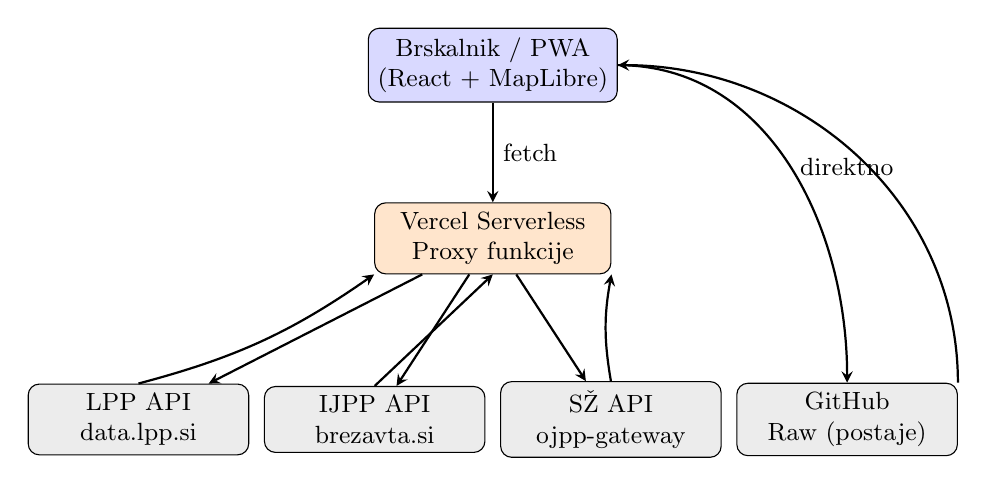
\begin{tikzpicture}[
  font=\small,
  box/.style={draw, rounded corners, minimum width=3cm, minimum height=0.8cm, align=center},
  api/.style={draw, rounded corners, minimum width=2.8cm, minimum height=0.8cm, align=center, fill=gray!15},
  arr/.style={->, >=stealth, thick}
]
% Client
\node[box, fill=blue!15] (client) at (0, 0) {Brskalnik / PWA\\(React + MapLibre)};

% Proxy layer
\node[box, fill=orange!20] (proxy) at (0, -2.2) {Vercel Serverless\\Proxy funkcije};

% APIs
\node[api] (lpp) at (-4.5, -4.5) {LPP API\\data.lpp.si};
\node[api] (ijpp) at (-1.5, -4.5) {IJPP API\\brezavta.si};
\node[api] (sz) at (1.5, -4.5) {SŽ API\\ojpp-gateway};
\node[api] (gh) at (4.5, -4.5) {GitHub\\Raw (postaje)};

% Arrows
\draw[arr] (client) -- node[right, align=left] {fetch} (proxy);
\draw[arr] (proxy) -- node[below left] {} (lpp);
\draw[arr] (proxy) -- (ijpp);
\draw[arr] (proxy) -- (sz);
\draw[arr] (client.east) to[out=0,in=90] node[right] {direktno} (gh.north);
\draw[arr] (lpp.north) to[bend right=10] (proxy.south west);
\draw[arr] (ijpp.north) -- (proxy.south);
\draw[arr] (sz.north) to[bend left=10] (proxy.south east);
\draw[arr] (gh.north east) to[out=90,in=0] (client.east);
\end{tikzpicture}
\caption{Visokonivojska arhitektura aplikacije IJPP Tracker}
\label{fig:arch}
\end{figure}

Ločevanje odjemalske in strežniške plasti zagotavlja, da je vsa logika prikaza in obdelave podatkov na strani odjemalca, medtem ko strežniška plast služi zgolj kot posrednik pri zahtevah, ki jih brskalniki sicer blokirajo zaradi varnostnih politik CORS. Statični podatki, kot so seznami postaj in poti linij, so shranjeni na platformi GitHub v obliki JSON datotek in jih aplikacija pridobi neposredno brez proxy posrednika, saj ta endpoint dovoljuje CORS dostop.

\subsection{Odjemalska stran - React SPA}

Odjemalska aplikacija je organizirana v hierarhijo komponent, pri čemer je korenski element komponenta \texttt{App}, ki upravlja globalno stanje in koordinira izmenjavo podatkov med zavihki. Navigacijo med štirimi glavnimi razdelki (zemljevid, postaje, linije,nastavitve) zagotavlja knjižnica React Router z načinom hash routing-a, ki je primeren za statično gostovanje na platformah brez podpore za strežniško usmerjanje.

Komponente zavihkov so naložene z leno inicializacijo (\texttt{React.lazy}), kar pomeni, da se koda posameznega zavihka prenese šele ob prvem obisku tega zavihka. S tem se skrajša čas do prve interaktivnosti aplikacije.

\subsection{Strežniška plast -- Vercel brezstrežniške funkcije}

Mapa \texttt{api/} vsebuje šest JavaScript datotek, ki se ob namestitvi na Vercel samodejno pretvorijo v HTTP-končne točke. Vsaka datoteka sledi vzorcu CORS-posrednika:
\begin{itemize}[noitemsep]
\item sprejme zahtevo od odjemalca,
\item jo posreduje ciljnemu API-ju,
\item doda ustrezne glave \texttt{Access-Control-Allow-Origin},
\item vrne odgovor odjemalcu.
\end{itemize}

Funkcije so implementirane v dveh izvajalnih okoljih (runtime).

Nekatere, na primer \texttt{lpp-arrivals.js}, so konfigurirane kot \texttt{runtime: "nodejs"}. To je potrebno, ker vsebujejo logiko za ponovitev zahteve ob napaki in predpomnjenje. Druge, na primer \texttt{lpp-stops.js}, pa so konfigurirane kot \texttt{runtime: "edge"}, kar pomeni izvajanje v globalni mreži robnih vozlišč z nižjo latenco, a brez dostopa do polnega Node.js API-ja.

\subsection{Upravljanje stanja aplikacije}

Globalno stanje aplikacije je centralizirano v komponenti \texttt{App} in zajema: seznam postajališč (\texttt{busStops}, \texttt{szStops}), trenutne položaje vozil (\texttt{gpsPositions}, \texttt{trainPositions}), aktivno postajališče (\texttt{activeStation}), prihode za aktivno postajališče (\texttt{lppArrivals}, \texttt{ijppArrivals}, \texttt{szArrivals}), izbrano vozilo (\texttt{selectedVehicle}) in nastavitve vidnosti plasti na zemljevidu (\texttt{visibility}, \texttt{busOperators}).

Trajnost stanja med sejami je zagotovljena s shranjevanjem v \texttt{localStorage} brskalnika, kjer se ob vsaki posodobitvi zapišejo nastavitve teme, aktivno postajališče, nastavitve na zemljevidu prikazanih slojev in seznam priljubljenih postajališč.

\section{Podatkovni sloj - modul \texttt{Api.jsx}}

\subsection{Pregled modula}

Datoteka \texttt{src/Api.jsx} je osrednji podatkovni sloj aplikacije in obsega dobrih 700 vrstic kode. Vsebuje vse funkcije za pridobivanje podatkov iz zunanjih virov, logiko za predpomnjenje, pomožne funkcije za formatiranje časovnih podatkov ter algoritme za dekodiranje geografskih poti in interpolacijo položajev vozil.

\subsection{Mehanizem predpomnjenja}

Aplikacija implementira lastno dvoplastno shemo predpomnjenja, ki sledi različnim veljavnostim podatkov glede na njihovo naravo:

\begin{table}[h!]
\centering
\caption{Veljavnost predpomnjenih podatkov glede na tip}
\begin{tabular}{lll}
\toprule
\textbf{Tip podatkov} & \textbf{Veljavnost} & \textbf{Utemeljitev} \\
\midrule
Postajališča & 5 minut & Statični podatki, redko se spreminjajo \\
Položaji vozil & 5 sekund & Sprotni podatki \\
Prihodi & 15 sekund & Posodabljanje napovedi prihodov \\
Poti (routes) & 5 minut & Geometrija poti se ne spreminja med vožnjo \\
\bottomrule
\end{tabular}
\label{tab:cache}
\end{table}

Splošno predpomnjenje zagotavlja objekt \texttt{Map} z imenom \texttt{cache}, ki za vsak URL ali ključ hrani par (podatki, časovni žig). Ločen objekt \texttt{routeCache} skrbi za predpomnjenje geometrij in postajališč posameznih voženj. Objekt \texttt{routeInFlight} pa preprečuje podvajanje sočasnih zahtev za isto vožnjo - če zahteva za dani \texttt{tripId} že poteka, nova zahteva vrne obstoječo obljubo (Promise), namesto proženja nove HTTP zahteve.

\subsection{Normalizacija prihodov}

Trije podatkovni viri prihodov vračajo čase v različnih formatah: LPP API vrača koliko minut je še do prihoda (\texttt{eta\_min}), IJPP API vrača sekunde od polnoči, SŽ API pa vrača ISO 8601 časovne žige. Funkcija \texttt{computeEtaAndTime} normalizira vse tri formate v enoten par (minute do prihoda, ura v formatu HH:mm):

\begin{lstlisting}[caption={Normalizacija ETA iz različnih formatov}, label={lst:eta}]
function computeEtaAndTime(arrival) {
	let etaMin = arrival.etaMinutes ?? arrival.eta_min ?? undefined;
	let actualTime =
		arrival.realtimeDeparture ||
		arrival.actualDeparture ||
		arrival.scheduledDeparture ||
		arrival.estimated_arrival_time ||
		arrival.arrival_time ||
		arrival.realtimeArrival ||
		arrival.scheduledArrival;

	let actualDate = null;
	if (actualTime) {
		actualDate = new Date(actualTime);
		// If parsing failed or if it looks like a time-only string, try prepending today's date
		if (
			isNaN(actualDate.getTime()) &&
			typeof actualTime === "string" &&
			actualTime.match(/^\d{2}:\d{2}(:\d{2})?$/)
		) {
			const today = new Date().toISOString().split("T")[0];
			actualDate = new Date(`${today}T${actualTime}`);
		}
	}
	if (actualDate && isNaN(actualDate.getTime())) {
		actualDate = null;
	}

	// Generate ETA if missing
	if (etaMin === undefined && actualDate) {
		const now = new Date();
		etaMin = Math.max(
			0,
			Math.round((actualDate.getTime() - now.getTime()) / 60000),
		);
	}

	// Generate actual time if missing
	if (!actualDate && etaMin !== undefined) {
		actualDate = new Date(new Date().getTime() + etaMin * 60000);
	}

	const timeStr = actualDate ? formatTime(actualDate) : "N/A";
	return {
		etaMinutes: etaMin ?? undefined,
		arrivalTime: timeStr,
	};
};

\end{lstlisting}

Funkcija \texttt{seconds2time} pretvori sekunde od polnoči v niz \texttt{HH:MM:SS}, kar je potrebno za obdelavo odgovorov IJPP API-ja, ki čase vrača v tej obliki.

\subsection{Pridobivanje položajev vozil}

Aplikacija sočasno pridobiva položaje mestnih avtobusov LPP in medkrajevnih avtobusov IJPP z vzporednimi klici prek \texttt{Promise.all}. Oba seznama se nato združita v enoten niz, ki se posreduje komponentam za prikaz.

LPP API vrača objekte z lastnostmi \texttt{latitude}, \texttt{longitude}, \texttt{line\_number} in \texttt{trip\_id}.

IJPP API vrača objekte v drugačni strukturi z gnezdenimi polji:
\texttt{vehicle.operator\_name}, \texttt{trip\_headsign} in \texttt{stop.name}.

Obe strukturi se v funkcijah \texttt{fetchLPPPositions} in \texttt{fetchIJPPPositions} prevedeta v enoten format z lastnostmi \texttt{gpsLocation}, \texttt{operator}, \texttt{lineName} in \texttt{tripId}.

\subsection{Sledenje vlakom z interpoliranjem položaja}

Sledenje vlakom je tehnično zahtevnejše kot sledenje avtobusom, saj SŽ API ne oddaja dejanskih položajev vlakov s frekvenco, primerno za tekoče gibanje na karti. Rešitev temelji na predhodnem računanju celotne poti vlaka s časovnimi žigi in naknadnim interpoliranju položaja na osnovi sistemskega časa.

Funkcija \texttt{fetchTrainPositions} pridobi vse aktivne vlake v oknu 60 sekund. Vsak vlak vsebuje pot v kodirani obliki Polyline in čase odhoda ter prihoda. Iz teh podatkov se zgradi tabela točk z absolutnimi časovnimi žigi:

\begin{lstlisting}[caption={Gradnja časovno označene poti vlaka}, label={lst:trainpath}]
// Izracunaj razdalje med tockami z Haversine formulo
let totalDist = 0;
const dists = [0];
for (let i = 1; i < coords.length; i++) {
  totalDist += haversine(coords[i-1], coords[i]);
  dists.push(totalDist);
}
// Vsaki tocki pripisemo casovni zig glede na delno razdaljo
path = coords.map((coord, i) => ({
  coord,
  time: adjDep + (dists[i] / totalDist) * duration
}));
\end{lstlisting}

\begin{sloppypar}
Animacijska zanka v komponenti \texttt{App} teče s frekvenco 1\,Hz z \mbox{\texttt{requestAnimationFrame}}.

Ob vsakem ciklu se za vsak vlak pokliče funkcija \texttt{getInterpolatedPosition}. Ta interpolira položaj in smer gibanja (bearing):
\end{sloppypar}

\begin{lstlisting}[caption={Interpolacija položaja vlaka na poti}, label={lst:interp}]
for (let i = 1; i < path.length; i++) {
  if (now <= path[i].time) {
    const prev = path[i - 1];
    const curr = path[i];
    const t = (now - prev.time) / (curr.time - prev.time);
    const coord = [
      prev.coord[0] + (curr.coord[0] - prev.coord[0]) * t,
      prev.coord[1] + (curr.coord[1] - prev.coord[1]) * t
    ];
    return { coord, bearing: calcBearing(prev.coord, curr.coord) };
  }
}
\end{lstlisting}

\section{Kartografski prikaz}

\subsection{Knjižnica MapLibre GL}

Osnova za kartografski prikaz je knjižnica MapLibre GL JS \cite{maplibre}, odprtokodna nadgradnja projekta Mapbox GL JS. Knjižnica za upodabljanje zemljevida uporablja tehnologijo WebGL, kar zagotavlja tekoče gibanje in visoko zmogljivost celo pri prikazu tisočih točk hkrati. Karti sta dve: svetla (OpenStreetMap Raster Light) in temna (OpenStreetMap Raster Dark), med njima pa lahko preklopi uporabnik.

\subsection{Organizacija slojev karte}

Kartografski prikaz je organiziran v module znotraj mape \texttt{src/tabs/map/}:

\begin{table}[h!]
\centering
\caption{Moduli kartografskega prikaza}
\begin{tabular}{ll}
\toprule
\textbf{Datoteka} & \textbf{Odgovornost} \\
\midrule
\texttt{config.js} & Konstante, ikone, barvne sheme prevoznikov \\
\texttt{layers.js} & Dodajanje in posodabljanje GeoJSON virov in slojev \\
\texttt{interactions.js} & Pojavna okna (popup) ob kliku na vozilo/postajališče \\
\texttt{popups.js} & HTML predloge za vsebino pojavnih oken \\
\texttt{utils.js} & Pretvorba podatkov v GeoJSON format \\
\bottomrule
\end{tabular}
\label{tab:mapmodules}
\end{table}

Vsaka entiteta na karti je urejena v plast (\textit{layer}), ki je vezana na vir podatkov (\textit{source}) tipa GeoJSON. Avtobusi, postajališča, vlaki in železniške postaje so ločeni sloji, kar omogoča neodvisno vklapljanje in izklapljanje posameznih slojev zemljevida.

\subsection{Gruče postajališč in avtobusov}

Postajališča in avtobusi so pri nižji stopnji povečave prikazani v obliki gruč (cluster). Ko je elementov preveč za pregleden prikaz, se samodejno združijo v krog s številko, ki pove, koliko jih je v skupini. Z večanjem povečave se gruče razpustijo v posamezna postaje in avtobuse.

\subsection{Prikaz izbrane poti}

Ob izbiri vozila iz kateregakoli zavihka se na karti izriše celotna trasa linije s postajišči. Trasa je prikazana kot linijski sloj na vrhu vseh ostalih slojev, postajišča na trasi pa so označena s krogi, ki so barvno usklajeni z barvno shemo prevoznika. Komponenta \texttt{RouteTab} prikaže predal s podrobnostmi o vsakem postajališču, vključno z predvidenimi časi prihodov.

\subsection{Prilagodljiva frekvenca osveževanja}

Frekvenca pridobivanja podatkov o položajih avtobusov je dinamično prilagojena stopnji povečave karte (zoom level):

\begin{table}[h!]
\centering
\caption{Frekvenca osveževanja glede na stopnjo povečave}
\begin{tabular}{lll}
\toprule
\textbf{Stopnja povečave} & \textbf{Interval} & \textbf{Utemeljitev} \\
\midrule
Pod 10 & 15 sekund & Majhna gostota informacij \\
10--11 & 10 sekund & Zmerna podrobnost \\
12--13 & 5 sekund & Visoka podrobnost \\
14 in več & 2 sekundi & Kar se da sprotno posodabljanje informacij \\
\bottomrule
\end{tabular}
\label{tab:polling}
\end{table}

Dodatno je osveževanje zaustavljeno, kadar je zavihek brskalnika v ozadju (zaznano prek \texttt{document.addEventListener("visibilitychange", ...)}), in obnovljeno ob vrnitvi v ospredje. S tem se zmanjša obremenitev API-jev in varčuje z baterijo na mobilnih napravah.

\section{Uporabniški vmesnik}

\subsection{Zavihek Postaje}

Zavihek \texttt{StationsTab} omogoča iskanje postajališč po imenu in prikaz najbližjih glede na lokacijo uporabnika. Implementiran je v treh pogledih: \textit{V bližini} (privzeto), \textit{Vsa postajališča} in \textit{Priljubljena}.

Za zmogljivo prikazovanje dolgih seznamov, ki so pogosto dolgi več tisoč vnosov, je uporabljena tehnika virtualiziranega izrisovanja prek knjižnice \texttt{react-window}. Komponenta \texttt{VariableSizeList} izrisuje samo tiste vrstice, ki so dejansko vidne v pogledu (viewport), kar drastično zmanjša število DOM (Document Object Model) elementov in izboljša zmogljivost.

Priljubljena postajališča so shranjena v \texttt{localStorage} in so dostopna tudi brez omrežne povezave. Razdalja od uporabnika je izračunana z Haversine formulo in prikazana poleg vsakega postajališča.

\subsection{Zavihek Linije}

Zavihek \texttt{LinesTab} prikazuje prihode za izbrano postajališče, ločeno po virih (LPP, IJPP, SŽ), ter seznam vseh aktivnih linij, pridobljenih iz GPS podatkov. Omogoča iskanje linij po imenu in označevanje priljubljenih linij.

Ob kliku na prihod ali linijo se prikliče funkcija \texttt{getTripFromId}, ki pridobi podrobnosti o vožnji in jih posreduje zemljevidu za prikaz trase. Prihodi so prikazani z ETA vrednostjo in absolutnim časom prihoda v formatu HH:mm.

\subsection{Zavihek Nastavitve}

Nastavitve omogočajo vklapljanje in izklapljanje posameznih slojev karte (avtobusi, avtobusna postajališča, vlaki, železniška postajališča) ter filtriranje prikazanih avtobusnih prevoznikov (Arriva, LPP, Nomago, Marprom, Prevozi Murska Sobota). Vse nastavitve se samodejno shranjujejo v \texttt{localStorage}.

\section{Izzivi med razvojem in rešitve}

\subsection{Neujemanje postajališč med podsistemi}

Eden najpomembnejših tehničnih izzivov je bilo dejstvo, da LPP, BrezAvta in sistema za identifikacijo postajališč ne uporabljata istih identifikatorjev. LPP ima lasten sistem šifer postajališč (\texttt{ref\_id}, \texttt{station\_code}), BrezAvta pa operira z identifikatorji, ki so skladni z GTFS standardom (\texttt{gtfs\_id}).

Izziv: postajališče Trzin - Zalog je v bazi LPP označeno z \texttt{ref\_id = 6201045}, v IJPP sistemu pa z \texttt{gtfs\_id = "lpp:6201045"}.

Rešitev: za vsako postajališče se vzdržuje objekt z več identifikatorji:

\begin{lstlisting}[caption={Interni objekt postajališča z identifikatorji vseh sistemov}, label={lst:stop}]
return {
  ...stop,
  name: stop.name ?? stop.stop_name ?? "",
  gpsLocation: gpsLocation,
  ref_id: refId,        // LPP identifikator
  ijpp_id: ijppId,      // IJPP identifikator
  gtfs_id: stop.gtfs_id, // GTFS identifikator
  stopId: stop.stopId,  // SZ identifikator
  routes_on_stop: routesOnStop, // seznam lpp linij, ki ustavljajo na postajališču
};
\end{lstlisting}

Ob pridobivanju prihodov aplikacija preveri, kateri identifikator je na voljo za aktivno postajališče, in pokliče ustrezen API:

\begin{lstlisting}[caption={Pogojno klicanje API-jev glede na razpoložljive identifikatorje}, label={lst:idcheck}]
// LPP prihodi
const lppCode = activeStation?.ref_id || activeStation?.station_code;
if (!lppCode) { setLppArrivals([]); return; }

// IJPP prihodi
const ijppId = activeStation?.gtfs_id;
if (!ijppId) { setIjppArrivals([]); return; }

// SZ prihodi
const szId = activeStation?.stopId;
// fetchSzArrivals vrne [] ce szId ni definiran
\end{lstlisting}

Osnova za ta mehanizem je enotna datoteka \texttt{unified\_stops\_with\_gtfs.json}, ki je naložena v repozitoriju \texttt{jakecernet/ijpp-json} na platformi GitHub. Ta datoteka je bila ročno sestavljena in (delno) prečiščena ter vsebuje preslikavo med identifikatorji vseh sistemov za vsako postajališče.

\subsection{Heterogenost podatkovnih vmesnikov}

Vsak od treh prometnih sistemov vrača podatke prek vmesnikov s povsem različnimi strukturami, avtentikacijo in obnašanjem.

LPP API zahteva, da ga naslavljamo prek Vercel proxy-ja, saj neposredni dostop iz brskalnika ni dovoljen. Vrača podatke v obliki \texttt{\{data: \{arrivals: [...]\}\}}, kjer so prihodi urejeni po \texttt{eta\_min}. API je razmeroma zanesljiv in dokumentiran.

IJPP API prek strežnika \texttt{api.beta.brezavta.si} vrača prihode za postajališče s parametrom \texttt{?current=true} v obliki \texttt{\{arrivals: [...]\}}, kjer so časi prihoda in odhoda v sekundah od polnoči.

SŽ API prek strežnika \texttt{mapper-motis.ojpp-gateway.derp.si} temelji na odprtokodnem sistemu MOTIS \cite{motis} za načrtovanje potovanj. Za prihode vrača strukturo \texttt{\{stopTimes: [...]\}} z gnezdenim objektom \texttt{place}, za geometrijo poti pa kodirani polyline z natančnostjo 6 decimalnih mest (namesto standardnih 5).

Rešitev je bila implementacija ločenih funkcij, ki normalizirajo izhod v enotno interno obliko.

Vse tri funkcije (\texttt{fetchLppArrivals}, \texttt{fetchIjppArrivals}, \texttt{fetchSzArrivals}) ob izhodu vrnejo tabelo objektov z istim naborom lastnosti: \texttt{etaMinutes}, \texttt{arrivalTime}, \texttt{tripName}, \texttt{tripId}, \texttt{realTime} in drugi.

\subsection{Dinamično posodabljanje URL-ja za pridobivanje položajev vlakov}

SŽ API za pridobivanje aktivnih vlakov zahteva časovno okno v parametrih URL-ja. Naslov vsebuje parametra \texttt{startTime} in \texttt{endTime} v formatu ISO 8601, ki morata biti ažurna ob vsakem klicu. Statičnega URL-ja, ki bi ga zgolj poklical vsakih $n$ sekund, ni mogoče definirati.

Izziv: standardna Fetch API v JavaScriptu pričakuje statičen niz URL-ja. Definicija konstantne spremenljivke za URL vlakov bi vedno vsebovala čas ob zagonu aplikacije, ne pa čas ob dejanskem klicu.

Rešitev: implementacija funkcije \texttt{buildSzLocationsLink()}, ki ob vsakem klicu dinamično zgradi URL z aktualnim časovnim oknom:

\begin{lstlisting}[caption={Dinamična gradnja URL-ja za SŽ API}, label={lst:dynurl}]
function buildSzLocationsLink() {
  const now = new Date();
  const later = new Date(now.getTime() + 60000); // +60 sekund
  return `https://mapper-motis.ojpp-gateway.derp.si/api/v1/map/trips` +
    `?min=49.41...&max=36.38...` +
    `&startTime=${encodeURIComponent(now.toISOString())}` +
    `&endTime=${encodeURIComponent(later.toISOString())}` +
    `&zoom=20`;
}
\end{lstlisting}

Namesto shranjene konstante se pri vsakem klicu \texttt{fetchTrainPositions()} pokliče \texttt{buildSzLocationsLink()}, ki vrne URL z vrednostmi, ki so glede na trenutni čas pravilne.

Funkcija \texttt{encodeURIComponent} poskrbi za pravilno kodiranje znakov, ki bi sicer povzročili napačno razčlenjevanje URL-ja (npr.\ dvopičje in plus v ISO 8601 formatu).

Dodatna zahteva API-ja je, da vsebuje bounding box (geografski pravokotnik) celotnega ozemlja, pokritega s slovenskim železniškim omrežjem. Ker SŽ API ponuja tudi lokacije vlakov za druge države, je v funkciji \texttt{fetchTrainPositions} implementiran filter po barvni kodi linije (\texttt{routeColor === "29ace2"}), ki ustreza barvni identiteti Slovenskih železnic.

\subsection{Dekodiranje poti vlakov}

SŽ API vrača geometrijo poti v kodirani obliki Polyline, ki je algoritem za kompresijo niza geografskih koordinat v ASCII niz \cite{polyline}. Standardna implementacija algoritma predvideva natančnost 5 decimalnih mest (faktor 1e5), SŽ API pa pri nekaterih poteh uporablja natančnost 6 decimalnih mest (faktor 1e6).

Rešitev: funkcija \texttt{decodePolylineToPoints} najprej dekodira niz z nastavljenim faktorjem. Če koordinate prve točke padejo izven veljavnega geografskega območja, samodejno preskusi z faktorjem 1e6:

\begin{lstlisting}[caption={Avto-zaznavno dekodiranje Polyline z variabilno natančnostjo}, label={lst:poly}]
export function decodePolylineToPoints(str, precision) {
  if (!str || typeof str !== "string") return [];
  let pts = decodePolylineOnce(str, precision);
  const first = pts[0];
  // Ce tocka ni v veljavnem obsegu, poskusi z vecjo natancnostjo
  if (!first || !isValidCoord(first)) {
    const alt = decodePolylineOnce(str, precision + 1);
    if (alt[0] && isValidCoord(alt[0])) pts = alt;
  }
  return pts.filter(isValidCoord);
}
\end{lstlisting}

\section{Namestitev in gostovanje}

\subsection{Orodje za gradnjo Vite}

Gradnja aplikacije poteka z orodjem Vite \cite{vite}, ki je sodobna alternativa klasičnim orodjem, kot sta Webpack in Parcel. Vite med razvojem izkorišča nativne ES module brskalnika za hitrejše posodabljanje brez ponovne gradnje celotne aplikacije. Za produkcijo Vite z orodjem Rollup ``pakira`` vso kodo in vire v optimizirane datoteke.

\subsection{Progresivna spletna aplikacija}

Aplikacija je konfigurirana kot PWA prek vtičnika \texttt{vite-plugin-pwa}. PWA je spletna aplikacija, ki jo je mogoče namestiti na domačo stran telefona ali namizja in deluje podobno kot nativna aplikacija \cite{pwa}. Konfigurirani so: servisni delavec (service worker) za predpomnjenje datotek, manifest z ikonami aplikacije v ločljivostih 192×192 in 512×512 pikslov ter meta oznake za podporo na napravah Apple iOS (\texttt{apple-mobile-web-app-capable}).

\subsection{Kontinuirano nameščanje}

Nameščanje aplikacije je avtomatizirano s skriptami v \texttt{package.json}: ukaz \texttt{npm run build} zgradi optimizirano različico, ukaz \texttt{npm run deploy} pa jo objavi na GitHub Pages prek paketa \texttt{gh-pages}. Vercel brezstrežniške funkcije se samodejno namestijo ob vsaki potisni objavi (push) v repozitorij.

\section{Zaključek}

Seminarska naloga je predstavila razvoj aplikacije IJPP Tracker, ki uspešno združuje podatke treh ločenih sistemov javnega potniškega prometa v Republiki Sloveniji v enoten spletni vmesnik s sprotnim sledenjem vozil.

Potrjeni sta bili dve od treh zastavljenih hipotez. Prvič, sodobne spletne tehnologije - konkretno React, MapLibre GL in ogrodje PWA - omogočajo vzpostavitev zmogljive aplikacije za sledenje javnemu potniškega prometa brez nativnega mobilnega razvoja; namestitev aplikacije na mobilno napravo kot PWA je funkcionalno enakovredna nativnim aplikacijam za ta namen. Drugič, razlike med podatkovnimi vmesniki posameznih sistemov je mogoče premostiti z abstrakcijsko plastjo v modulu \texttt{Api.jsx}, ki normalizira heterogene strukture v enotni interni format.

Tretja hipoteza - da varnostne politike CORS zahtevajo strežniški posredovalni sloj -- je bila prav tako potrjena: dva od treh podatkovnih virov (LPP in SŽ API) zahtevata posredovanje prek Vercel brezstrežniških funkcij.

Trije ključni izzivi, ki so bili identificirani in rešeni: (1) neujemanje identifikatorjev postajališč je bilo rešeno z ročno pripravljeno enotitveno datoteko \texttt{unified\_stops\_with\_gtfs.json}; (2) heterogenost podatkovnih vmesnikov je bila naslovljena z normalizacijskim slojem in ločenimi funkcijami za vsak sistem; (3) dinamično posodabljanje URL-ja za SŽ API je bilo rešeno s funkcijo, ki ob vsakem klicu zgradi aktualni naslov.

Med razvojem je bilo ugotovljeno, da dostopnost in stabilnost javnih API-jev ostajata izziv: IJPP API vzdržuje ekipa prostovoljcev, prav tako SŽ API, kar pomeni, da lahko pride do občasnih nedostopnosti ali sprememb v strukturi podatkov, ki zahtevajo prilagoditve v aplikaciji. 

\newpage
\begingroup
\makeatletter
\section{Viri in literatura}
\nocite{*}
\printbibliography[heading=none]
\makeatother
\endgroup

\newpage
\begin{samepage}
    \thispagestyle{empty}
    \section*{Izjava o avtorstvu}
    Izjavljam, da je seminarska naloga z naslovom \textit{IJPP Tracker - spletna aplikacija za sledenje javnega potniškega prometa v Republiki Sloveniji} v celoti moje avtorsko delo, ki sem ga izdelal samostojno s pomočjo navedene literature in pod vodstvom mentorja.

    \vfill

    \today \hfill Jaka Černetič
    \vspace{3cm}
\end{samepage}

\end{document}
